\subsection{\Acp{rltanlage} Vergangenheit}
Lüftungsgeräte sind schon seit längerer Zeit in Verwendung \zB in Wirtschaftsbetrieben, Gastronomie aber auch in Bürogebäuden. Die Ursprünge von Lüftungsgeräten bzw. \ac{rltanlage} lassen sich jedoch schon auf ca. 3000 v. Chr. datieren.
Die ersten Versuche fanden dahingehen Anwendung, um Höhlen und Unterkünfte vom Rauch des Feuers zu befreien. Es wurden solche Arten von Raumbelüftungen \zB in Ondol in Alaska gefunden.
Lüftungstechnik wurde damals durch den natürlichen Wetterzyklus bestimmt. 
Erst im späteren Verlauf wurde durch die Entwicklung moderner Belüftungs- und Klimatechnik, die aktive Belüftung- und Temperaturregelung möglich gemacht.

Die ersten Gehversuche einer voll funktionsfähigen \acs{rltanlage} wurde 1836 im House of Commons in London gemacht. Die Anlage umfasst alle Punkte einer \acs{rltanlage} darunter zählen das Heizen, Kühlen, Be- und Entfeuchten sowie Filtern der Luft. Das zurückführen der Wärmeenergie von der \gls{abluft} zur \gls{zuluft} wie es heute in modernen \acp{rltanlage} der Fall ist, konnte damals technisch noch nicht realisiert werden.

Die folgende Beschreibung bezieht sich auf
Abb.~\ref{fig:House_of_Commons_Klimatechnik}.
Die Anlage versorgte das House of Commons mit \gls{aussenluft} welche links unten bei den Gitter angesaugt wird (Die Ansaugung der Frischluft lag knapp über der Themse). Die Kühlung wurde durch Eis welches in der Kammer hinter den Gittern liegt realisiert.
Die Filterung der \gls{aussenluft} wurde durch Baumwolle, welche im Bereich von Punkt C aufgeschichtet wird realisiert.
Nach der Filterung wurde im Winter bei Punkt A die \gls{zuluft} erhitzt. 
Danach strömte die \gls{zuluft} durch den doppelten Boden und wurde dadurch verteilt. Die Luft strömte nun nach oben durch das Gebäude und wurde bei Punkt F aus dem Gebäude geleitet. Im Winter leitete man die \gls{abluft} nach links direkt aus dem Fenster. Im Sommer hingegen wurde die \gls{abluft} nach rechts durch die Verrohrung und durch den Kamin  nach draußen geleitet. Zudem wurde im Kamin ein sogenanntes "Lockfeuer" gemacht, um der zuvor abströmenden \gls{abluft} den nötigen Auftrieb zu verleihen.
\cite[vgl.][]{Fitzner_Finke:2010}

\begin{figure}[ht]
	\centering
	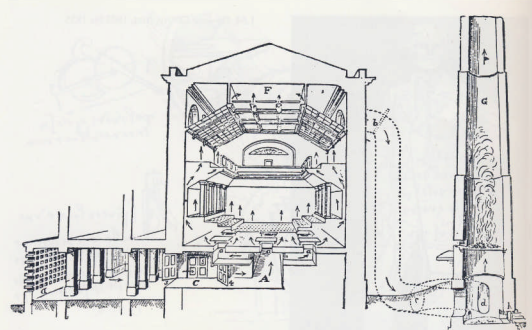
\includegraphics[width=1\linewidth]{Bilder/Belueftung_House_of_Commons}
	\caption{Klimatechnik House of Commons  (Quelle: \url{https://vhkk.org/page/vortrag/pdf/Geschichte_Raumklimatechnik.pdf})}
	\label{fig:House_of_Commons_Klimatechnik}
\end{figure}



\subsection{\Acp{rltanlage} Gegenwart}
Der Zweck einer \ac{rltanlage} heute, unterscheidet sich generell nicht viel von dem was auch schon \zB 1836 im House of Commons in London verwendet wurde. Die einzelnen Abschnitte wie \zB Ansaugung, Filtration, Be- und Entfeuchtung, Kühlung, Heizung und Absaugung der Luft hingegen, haben sich grundlegend geändert. So werden heutzutage durch die Verwendung von neuen Technologien und technischen Möglichkeiten die \acp{rltanlage} vollkommen anders Geplant und umgesetzt in deren Funktion.

Der Aufbau hat sich dahingehend restrukturiert, dass eine moderne \ac{rltanlage} sehr kompakt im Aufbau ist. Angefangen bei den Steuerungsklappen für Zu- bzw. \gls{abluft} über die Ventilatoren, das Heiz- bzw. Kühlregister, das Wärmerückgewinnungsregister, die Filter und der Luft Be- und Entfeuchter, ist alles in einer kompakten \ac{rltanlage} untergebracht. Auch was die zuvor angesprochenen Technologien angeht, wird heute schon lange nicht mehr auf Eis als Kühlmittel oder ein "Lockfeuer" für den Auftrieb der Luft eingesetzt. Diese Bereiche werden \zB von modernen Kühl- und Heizregistern übernommen und Ventilatoren sorgen für den benötigten Luftstrom in der \ac{rltanlage}. Doch nicht nur im inneren einer \ac{rltanlage} hat sich vieles geändert, auch Außen geht man einem völlig neuen Konzept nach. Da die meisten \acp{rltanlage} draußen installiert werden muss die Verkleidung und die Standfestigkeit den Umständen angepasst werden. Genauere Beschreibung in \ref{entwicklungs_rlt}.
Im folgenden werden die Komponenten anhand des allgemeinen Aufbauplans einer \ac{rltanlage} Abb.~\ref{fig:Aufbau_Lueftungsgerät_allgemein} beschrieben. 

\subsection{\Acp{rltanlage} allgemein}

\begin{figure}[H]
	\centering
	\includegraphics[width=1\linewidth]{Bilder/Lueftungsgerät_allgemein_aufbau}
	\caption{Allgemeiner Aufbau einer modernen \ac{rltanlage} (Quelle: \url{https://www.baunetzwissen.de/gebaeudetechnik/fachwissen/lueftung/bestandteile-von-lueftungsanlagen-2473103})}
	\label{fig:Aufbau_Lueftungsgerät_allgemein}
\end{figure}

\begin{itemize}
	\item \textbf{Ventilatoren}: In einer \ac{rltanlage} ist immer mindestens ein Ventilator vorhanden (abhängig der Größe der \ac{rltanlage}). Dieser ist für die Beförderung von Luftmassen durch die \ac{rltanlage} sowie die Beförderung aus und in das Gebäude zuständig. Der Ventilator muss mit Bedacht dimensioniert sein, da dieser in der \ac{rltanlage} den höchsten Stromverbrauch hat. Die Dimensionierung muss so gewählt werden, dass der intern herrschende Strömungswiderstand überwindet wird. Es gibt verschiedene Arten von Ventilatoren 
\begin{itemize}
	\item Axialventilatoren mit/ohne Leitrad Abb.~\ref{fig:EBM_Axialventilator}
	\item Radialventilatoren mit Laufräder (vorwärts- oder rückwertsgekrümmte Schaufeln)
	\item Querstrom- oder Tangentiallüfter 
\end{itemize}

\begin{figure}[H]
	\centering
	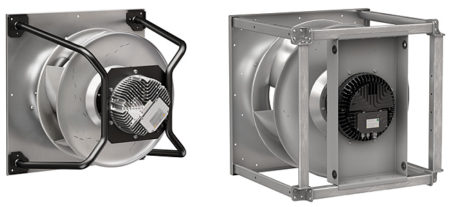
\includegraphics[width=0.5\linewidth]{Bilder/axialventilator}
	\caption{EBM Axialventilator} 
	(Quelle: \url{https://ebmpapst-7237.kxcdn.com/de/files/2017/11/RadiPac-mit-oder-ohne-tragspinne-450x207.jpg})
	\label{fig:EBM_Axialventilator}
\end{figure}

	\item \textbf{Heiz- und Kühlregister}: im Heiz- und Kühlregister Abb.~\ref{fig:heizregister} wird die einströmende Luft je nach Bedürfnis erhitzt oder gekühlt. Dies wird durch unterschiedlichste Heiz- oder Kühlmedien realisiert bsp. Dampf, heißes oder kaltes Wasser, welches durch das Heiz- bzw. Kühlregister fließt. Andere Arten um die einströmende Luft zu erhitzen sind: Elektrolufterhitzer, gasbetriebene Lufterhitzer. Um die Luft abzukühlen kann auch ein Direktverdampfer verwendet werden.
	Um Energiekosten zu sparen, wird der \gls{abluft} die Wärmeenergie entzogen und der \gls{zuluft} wieder hinzugefügt, dabei werden bis zu 98 Prozent der Wärmeenergie zurückgewonnen. Im Vergleich zu \ac{rltanlage} ohne Wärmerückgewinnung werden bis zu 30 Prozent an Heizenergie eingespart. 

\begin{figure}[H]
	\centering
	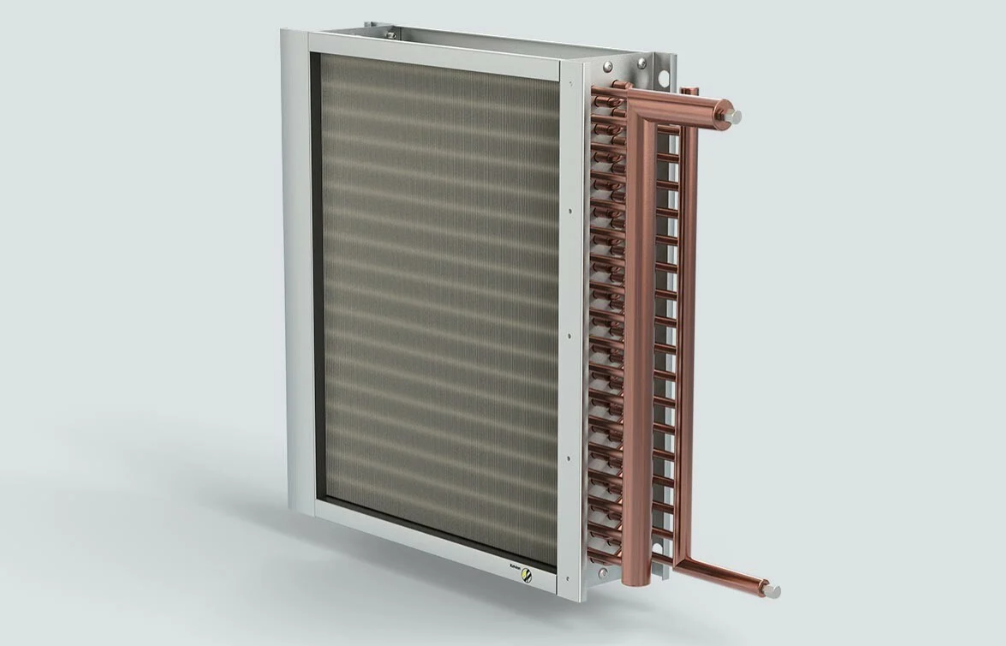
\includegraphics[width=0.5\linewidth]{Bilder/luftwaermeregister}
	\caption{Heiz- Kühlregister} 
	(Quelle: \url{https://www.baunetzwissen.de/gebaeudetechnik/fachwissen/lueftung/bestandteile-von-lueftungsanlagen-2473103/gallery-1/5})
	\label{fig:heizregister}
\end{figure}

	\item \textbf{Luft Be- und Entfeuchter}: Der Luft Be- und Entfeuchter Abb.~\ref{fig:luftbefeuchter} ist dafür zuständig, dass die \gls{zuluft} und dessen Luftfeuchtigkeit den Sollwert nicht unter- bzw. überschreiten. Meist wird für diesen Schritt ein Umlaufsprühbefeuchter eingesetzt. Dieses Bauteil ist jedoch zwecks dessen Hygiene, sehr Wartungsintensiv. 

\begin{figure}[H]
	\centering
	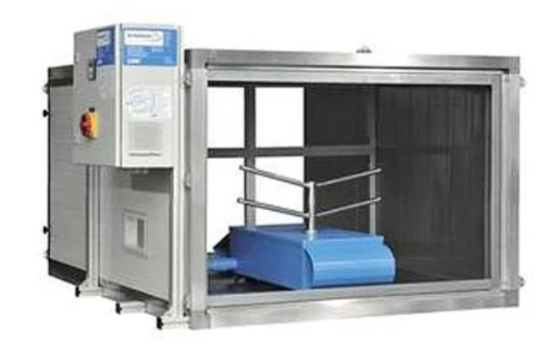
\includegraphics[width=0.5\linewidth]{Bilder/Luftbefeuchter}
	\caption{Luftbe- und Entfeuchter} 
	(Quelle: \url{	https://www.baunetzwissen.de/gebaeudetechnik/fachwissen/lueftung/bestandteile-von-lueftungsanlagen-2473103/gallery-1/6})
	\label{fig:luftbefeuchter}
\end{figure}

\item \textbf{Filter}: Die verbauten Filter sind für die Filterung der \gls{aussenluft} zuständig. Filter werden laut der DIN EN ISO 16890-1 in 3 Gruppen unterteilt.
\begin{itemize}
	\item PM (Particulate Matter) 1: Partikel die größer als 1 Mikrometer sind \zB Viren oder Verbrennungspartikel 
	\item PM (Particulate Matter) 2,5: Partikel die größer als 2,5 Mikrometer sind \zB Bakterien oder Pilze
	\item PM (Particulate Matter) 10: Partikel die größer als 10 Mikrometer sind \zB Pollen oder Staub
\end{itemize}
Es werden zur Reinigung der \gls{aussenluft} entweder Taschenfilter Abb.~\ref{fig:taschenfilter} oder Kassettenfilter verwendet. Um Gerüche aus der Luft zu filtern \zB in Küchen werden Aktivkohlefilter verwendet. Bei beiden Filterarten ist es wichtig diese in regelmäßigen Abständen zu säubern oder ersetzten.  

\begin{figure}[H]
	\centering
	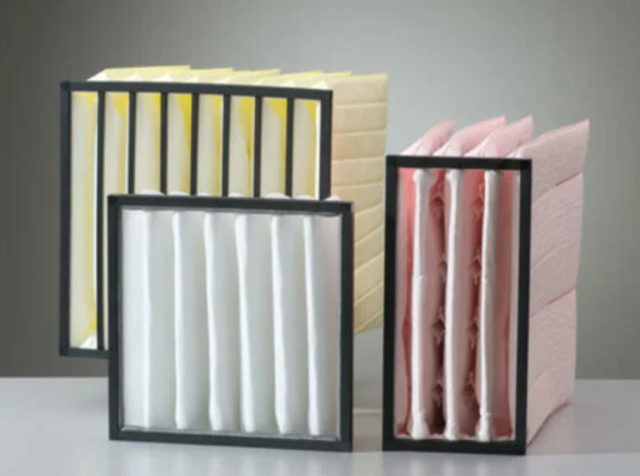
\includegraphics[width=0.5\linewidth]{Bilder/normalefilter}
	\caption{Taschenfilter} 
	(Quelle: \url{	https://www.baunetzwissen.de/gebaeudetechnik/fachwissen/lueftung/bestandteile-von-lueftungsanlagen-2473103/gallery-1/7})
	\label{fig:taschenfilter}
\end{figure}

	\item \textbf{Schalldämpfer}: Schalldämpfer Abb.~\ref{fig:schalldaempfer} sind für die Absorption von Lärmquellen in einem Lüftungsgerät zuständig. Die Lärmquelle mit dem höchsten Lärmpegel sind dabei die Ventilatoren. Es wird dabei unterschieden zwischen:
\begin{itemize}
	\item Absorptions-Schalldämpfer 
	\item Drossel-Schalldämpfer
	\item Resonanz-Schalldämpfer
\end{itemize} 
	Auch die richtige Anordnung und Dimensionierung der Verrohrung zwischen einzelnen Räumen, welche an der selben \ac{rltanlage} angeschlossen sind ist essenziell. Dabei werden Strömungsgeräusche (Geräusch welche zwischen zwei Räumen durch die Verrohrung transportiert werden) verhindern.

\begin{figure}[H]
	\centering
	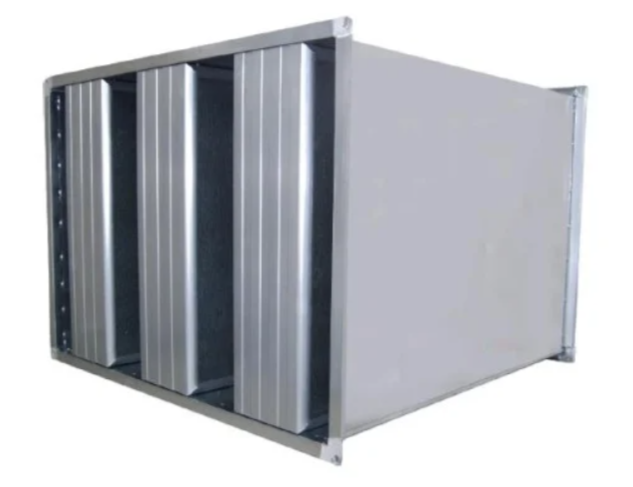
\includegraphics[width=0.5\linewidth]{Bilder/schalldaempfer}
	\caption{Schalldämpfer (Mineralwolle als Dämpfmaterial)} 
	(Quelle: \url{	https://www.baunetzwissen.de/gebaeudetechnik/fachwissen/lueftung/bestandteile-von-lueftungsanlagen-2473103/gallery-1/8})
	\label{fig:schalldaempfer}
\end{figure}

	\item \textbf{Drossel- und Jalousieklappen}: 
	Drossel- und Jalousieklappen Abb.~\ref{fig:drosselklappe} werden dahingehend eingesetzt, um durchgehend einen konstanten Volumenstromwert zu erreichen. 

\begin{figure}[H]
	\centering
	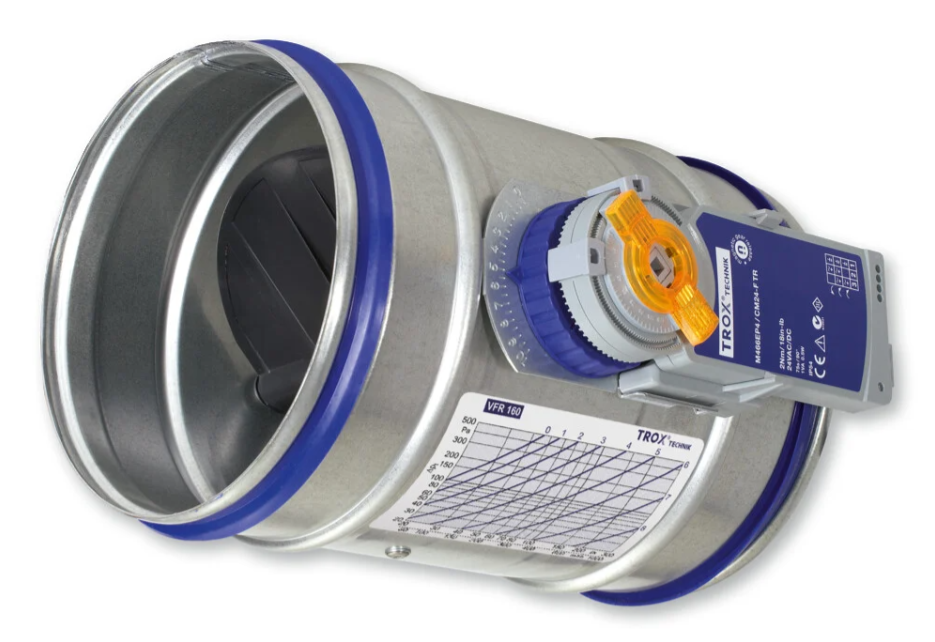
\includegraphics[width=0.5\linewidth]{Bilder/drosselklappe}
	\caption{Drosselklappe} 
	(Quelle: \url{	https://www.baunetzwissen.de/gebaeudetechnik/fachwissen/lueftung/bestandteile-von-lueftungsanlagen-2473103/gallery-1/10})
	\label{fig:drosselklappe}
\end{figure}

	\item \textbf{Volumenstromregler}: Der Volumenstromregler arbeitet eng mit den Drossel- und Jalousieklappen zusammen. Dabei wird zwischen einem Konstant-Volumenstromregler oder einem variablen Volumenstromregler. Wie aus dem Namen abzuleiten, ist dieser für die Messung und Regelung des Luftvolumens zuständig. 

\begin{figure}[H]
	\centering
	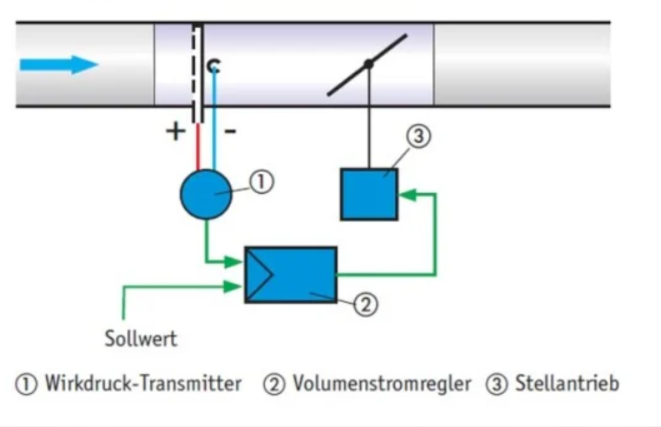
\includegraphics[width=0.5\linewidth]{Bilder/volumenstromregler}
	\caption{Volumenstromregler} 
	(Quelle: \url{	https://www.baunetzwissen.de/gebaeudetechnik/fachwissen/lueftung/bestandteile-von-lueftungsanlagen-2473103/gallery-1/12})
	\label{fig:volumenstromregler}
\end{figure}

	\item \textbf{Brandschutzklappen und Rauchschutzklappen}:
	Die Sicherheit vor Feuer und Rauch ist durch sogenannte Brand- und Rauchschutzklappen gegeben.
	Diese Art von Klappen verhindert das sich Rauch oder Feuer über die Lüftungsschächte/Verrohrung durch das Gebäude ausbreitet. Brandschutzklappen Abb.~\ref{fig:Brandschutzklappe} sind zwischen den einzelnen Brandabschnitten eines Gebäudes angebracht. Rauchschutzklappen Abb.~\ref{fig:Rauchschutzklappe} sind im inneren der Lüftungsleitungen angebracht, dadurch wird verhindert, dass Menschen giftige Dämpfe und Rauch einatmen. Sowohl die Brandschutzklappe als auch die Rauchschutzklappe, schließen im Notfall (Brand- oder Rauchentwicklung) automatisch.
\end{itemize}

\begin{figure}[H]
	\centering
	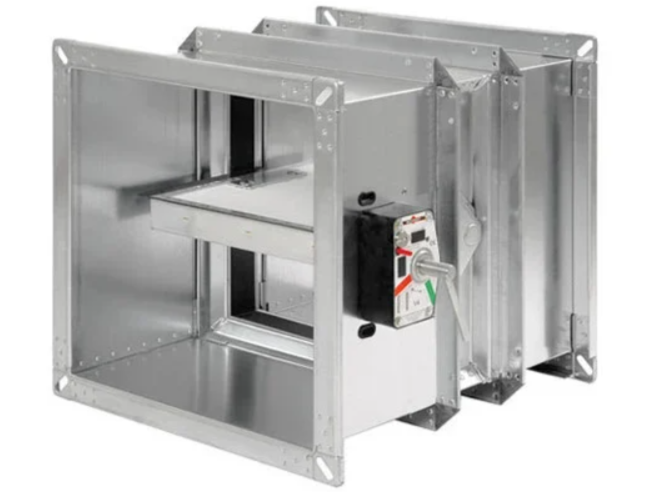
\includegraphics[width=0.5\linewidth]{Bilder/brandschutzklappe}
	\caption{Automatische Brandschutzklappe} 
	(Quelle: \url{	https://www.baunetzwissen.de/gebaeudetechnik/fachwissen/lueftung/bestandteile-von-lueftungsanlagen-2473103/gallery-1/14})
	\label{fig:Brandschutzklappe}
\end{figure}

\begin{figure}[H]
	\centering
	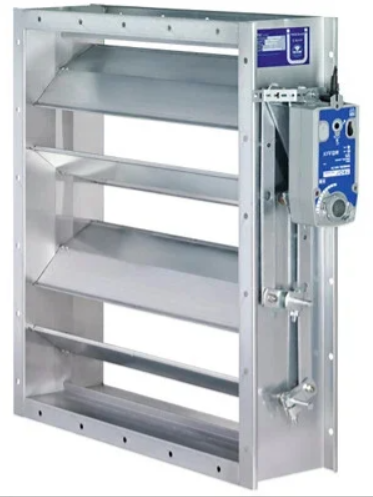
\includegraphics[width=0.5\linewidth]{Bilder/rauchschutzklappe}
	\caption{Rauchschutzklappe} 
	(Quelle: \url{	https://www.baunetzwissen.de/gebaeudetechnik/fachwissen/lueftung/bestandteile-von-lueftungsanlagen-2473103/gallery-1/15})
	\label{fig:Rauchschutzklappe}
\end{figure}

\cite[vgl.][]{baunetz_bestandteile_nodate:o.J.}

\subsection{\ac{rltanlage} Einsatzbereiche / Verwendungszweck}

\ac{rltanlage}n werden dahingehend eingesetzt um in Räumen oder Gebäuden die drei wichtigen Bereich der Raumlufttechnik abzudecken:

\begin{itemize}
	\item Lufttemperatur
	\item Luftfeuchtigkeit
	\item Luftqualität
\end{itemize} 

Dabei fördert die \ac{rltanlage} die verbrauchte Luft nach draußen. Die Luft wird bevor sie in die Umwelt gelassen wird gefiltert. Das ist wichtig, da die Luft welche in Industriebetrieben \zB einer Druckerei abgelassen wird, meist mit Schadstoffen versetzt sind. Diese Schadstoffe müssen abgelassen werden, da diese für den Menschen gesundheitsschädlich sein können. Durch das absaugen von Gefahrenstoffe aus der Luft, erhöht sich die Sicherheit der Mitarbeiter bezüglich der Gesundheit.

Durch die Speisung der frischer \gls{zuluft} und Absaugung der verbrauchten \gls{abluft} können Schadstoffpartikel, Viren und ein gewisses Maß an zu hoher oder zu niedriger Raumtemperatur und Raumluftfeuchtigkeit ausgeglichen werden. 
\cite[vgl.][]{DGWZ:o.J.}

Neben der vorher genannten Industrie werden \ac{rltanlage}n auch im medizinischen Sektor eingesetzt. In diesem Sektor wird der Fokus verstärkt auf die Luftqualität gelegt. Eine \ac{rltanlage} muss im medizinischen Sektor, zu jeder Zeit die Versorgung über die \gls{zuluft} mit frischem Sauerstoff gewährleistet sein. Die Abführung ist auch wichtig um verbrauchte (Kohlendioxyd haltige) Luft aus dem Operationssaal zu leiten. Zusätzlich muss im medizinischen Sektor der angeordnete Schutzbereich (\zB Operationssaal, Reinraum) besonders vor Kontamination geschützt werden. Dies wird meist mit einem leichten Überdruck gewährleistet, dass keine Kontamination (Viren etc.) mit außenliegender, nicht gefilteter Luft besteht.
\cite[vgl.][]{robatherm:2019,robatherm:o.J.}

Weitere Einsatzbereiche sind:
\begin{itemize}
	\item Labore
	\item Bürogebäude, Bildungsstätten (Schulen, Kindergarten)
	\item Küchen (Gastronomie)
	\item Verkaufsstätten
	\item Schwimmbäder
\end{itemize} 
\cite[vgl.][]{robatherm:2019,induux_wiki:2023}

\subsection{Entwicklungs- \ac{rltanlage} / \gls{tdot} \ac{rltanlage}}

Die Folgenden \acp{rltanlage} wurden von der Firma Walter Bösch GmbH für die Entwicklung einer \ac{rltanzeige} und dessen Präsentation an der HTL Dornbirn am TdoT, zur Verfügung gestellt. Bei beiden \acp{rltanlage} werden der Grundlegende Aufbau sowie die Funktionsweise beschrieben und dazu die jeweils verbauten Komponenten näher vorgestellt.

\subsection{Entwicklungs- \ac{rltanlage}} \label{entwicklungs_rlt}

\begin{figure}[H]
	\centering
	\includegraphics[width=1\linewidth]{Bilder/Lüftungsgerät_entwicklung}
	\caption{Entwicklungs- \ac{rltanlage}} 
	\label{fig:LG_entwicklung}
\end{figure}

\textbf{Funktionsweise / Aufbau:}

Bei der Entwicklungs- \ac{rltanlage} ist der Aufbau wie in der Abb.~\ref{fig:Bauplan_entwicklung} zu sehen, wie bei fast jeder \ac{rltanlage} in zwei größere Teile geteilt.
Beim (Punkt ODA) wird die noch ungefilterte \gls{aussenluft} in die \ac{rltanlage} eingespeist. Zuerst geht es durch die, je nach benötigter Luftmenge geöffneten, \gls{aussenluft} Klappe und anschließend durch die Filter um die \gls{aussenluft} von möglicher Verunreinigung zu reinigen. Danach wird durch die WRG-Klappe bestimmt ob die \gls{zuluft} am Wärmerückgewinnungsregister vorbei geleitet werden soll, oder ob dieses Durchströmt werden soll. Nach diesem Schritt geht es von links unten durch den Ventilator auf der linken Seite nach oben und dort durch das verbaute Heiz- und Kühlregister. Von dort (Punkt SUP) aus strömt die \gls{zuluft} nun durch die Verrohrung und verteilt sich im Gebäude. Die verbrauchte \gls{abluft} wird nun am (Punkt ETA) angesaugt und durch einen Filter gesogen (Reinigung der \gls{abluft} von \zB Fett oder Partikel). Danach wird die \gls{abluft} durch das Wärmerückgewinnungsregister geschleust um dieser Wärmeenergie zu entziehen (Erwärmung der \gls{zuluft}). Nach diesem Schritt wird die \gls{abluft} von rechts unten nach rechts oben durch den Ventilator befördert. Zum Schluss wird die \gls{abluft} durch die Fortluftklappe nach draußen gegeben. 

\begin{figure}[H]
	\centering
	\includegraphics[angle=90,width=0.7\linewidth]{Bilder/Aufbau_Lueftungsgerät_walter_boesch}
	\caption{Aufbau Entwicklungs- \ac{rltanlage}} 
	\label{fig:Bauplan_entwicklung}
\end{figure}


\textbf{Komponenten:}

Die ganze Entwicklungs- \ac{rltanlage} baut mit dessen Komponenten auf dem Modbus Protokoll auf. Dabei wird in dieser \ac{rltanlage} eine Parity von 19200 verwendet. Die ersten Bauteil welche die digitale Infrastruktur bilden sind die beide \gls{qbm}  (Siemens \gls{qbm}). Diese haben in dieser Ausbaustufe zwei Druckdifferezmesser welche je bis zu 1250Pa messen können. Damit misst man die Druckdifferenzen welche Aufschluss geben, wie verschmutzt die Filter sind (höherer Gegendruck).

Neben diesen Anschlüssen haben die \gls{qbm}  auch jeweils zwei Analog Input und Analog Output Ports. Die Analog Input Ports werden in erster Linie dafür benutzt um durch Temperatursensoren (LG-NI1000) einen Überblick zu bekommen welche Temperaturen im Gerät herrschen. Dabei liegt ein besonderes Augenmerk auf der \gls{zuluft} (Luft welche gereinigt ins Gebäude eingespeist wird) und der \gls{abluft} (welche das Gebäude nach draußen verlässt).

In dieser Konfiguration werden neben den Temperatursensoren für Zu- und \gls{abluft} auch noch weitere Temperatursensoren (LG-NI1000) verwendet. Diese sind zuständig für die Messwerte der \gls{aussenluft} und der Fortluft. All diese Temperatursensoren werden dabei ausgelesen und mit den Werten die die \gls{zuluft}, \gls{abluft}, \gls{aussenluft} und \gls{fortluft} ergeben, kann der Wärmerückgewinnungsgrad berechnet werden siehe Kapitel \ref{python_functions}. Zudem wird mit dem Temperatursensor welcher die \gls{aussenluft} misst die Frostschutz Temperatur bestimmt (verhindert einfrieren der Flüssigkeit im Heiz- und Kühlregister).

Mit den Analog Output Ports werden weitere Dinge gesteuert wie \zB die \gls{aussenluft}klappe. Diese Steuert die Luftzufuhr in die \ac{rltanlage}. Durch zufahren dieser Klappe wird die \ac{rltanlage} auch vor Witterung geschützt (die passiert Automatisch). Auch beim Analog Output angeschlossen ist die Wärmeregisterklappe. Wie zuvor schon erwähnt steuert diese den Durchfluss durch das Wärmerückgewinnungsregister (An heißen Tagen wird die Luft an der WRG-Klappe vorbei geführt um unnötiges erhitzen des Wärmerückgewinnungsregisters zu vermeiden).

Die Ventilatoren in der Entwicklungs- \ac{rltanlage} stammen von EBM. Es handelt sich dabei um zwei ebm-papst k3g310 Abb.~\ref{fig:ebmpapstventilator}. Diese sind in der \ac{rltanlage} für die Luft zu- und abfuhr zuständig. Die Ventilatoren können über das Modbus Protokoll direkt ausgelesen werden und damit können der aktuelle Soll- und Istwert der Drehzahl, sowie die Leistung und das Volumen (Luftvolumen Durchsatz) ausgegeben / berechnet werden. Einer der wichtigsten Angaben ist jedoch der Motorstatus, dieser zeigt an ob es aktuell Fehler im Betrieb der Ventilatoren gibt und wenn ja, welcher anliegt. siehe Kapitel \ref{python_functions}.

\begin{figure}[H]
	\centering
	\includegraphics[width=0.5\linewidth]{Bilder/ebmpapstventilator}
	\caption{ebm-papst k3g310-pt08-j2} 
	\label{fig:ebmpapstventilator}
\end{figure}

\textbf{Verkleidung:}

Wie man in Abb.~\ref{fig:LG_entwicklung} sieht. Ist die \ac{rltanlage} mit einem robusten Rahmen versehen, welcher mit leichten Aluminumplatten verkleidet wird. Die vorderen Klappen lassen sich leicht mit den Schwarzen Verschlüssen öffnen um einen leichteren Auf- und Zusammenbau sowie eine leichtere Wartung im Nachhinein zu garantieren. Zudem ist die \ac{rltanlage} in mehrere Segmente unterteilbar, das wiederum erleichtert einen leichteren Transport von sehr großen \acp{rltanlage}. Da die \ac{rltanlage} immer Witterungen ausgesetzt wird, ist sowohl die \ac{rltanzeige} sowie die gesamte \ac{rltanlage} Wasser- und Staubdicht. Um bei der Einrichtung des Gerätes Zeit und Kosten zu sparen sind alle wichtigen Anschlüsse dieser \ac{rltanlage} gut farblich und mit Schrift/Symbolen gekennzeichnet. 





\subsection{\gls{tdot} / Messe \ac{rltanlage}}

\textbf{Funktionsweise / Aufbau:}
\begin{figure}[H]
	\centering
	\includegraphics[width=0.7\linewidth]{Bilder/Lüftungsgerät_TdoT}
	\caption{\gls{tdot} / Messe \ac{rltanlage}} 
	\label{fig:LG_tdot}
\end{figure}

Beim der \gls{tdot} \ac{rltanlage} folgt der Aufbau und die Luftfließrichtung der Entwicklungs- \ac{rltanlage}. Auch hier wird die Luft oben bei der schwarzen \gls{aussenluft}klappe angesaugt, geht dann durch die Filter, das Wärmerückgewinnungsregister, den Ventilator und das Heiz- und Kühlregister in das Gebäude. Die \gls{abluft} wird auch auf dem selben Weg die die der Entwicklungs- \ac{rltanlage} nach draußen befördert. Die Luft wird bei der \gls{abluft}klappe (links über den beigen Pfeilen) angesogen, geht dann durch die Filter, das Wärmerückgewinnungsregister und den Ventilator durch die Fortluftklappe nach draußen. Durch die Veranschaulichung durch LED-Panels (LED-Pfeile) welche die Luftfließrichtung anzeigen, ist in dieser \ac{rltanlage} die Funktionsweise für den Laien leichter zu verstehen.

\textbf{Komponenten:}
In der \gls{tdot} \ac{rltanlage} wurde gleich wie in der Entwicklungs- \ac{rltanlage} eine Baudrate von 19200 für die Modbus Kommunikation vordefiniert. Auch in dieser \ac{rltanlage} kommen die von Siemens produzierten \gls{qbm} zu Einsatz. An diese werden wie schon zuvor bei der Entwicklungs- \ac{rltanlage} an den Analog Input Ports die Temperatursensoren für \gls{zuluft}, \gls{abluft} und \gls{fortluft} angeschlossen. Zudem wird auch hier mit dem Temperatursensor welcher die \gls{aussenluft} misst die Frostschutz Temperatur bestimmt. Die Klappensteuerung (\gls{aussenluft}klappen und WRG-Klappe0) übernehmen auch hier die Analog Output Ports zusätzlich dem WRG-Relais. Die Druckdifferenzen werden in der Entwicklungs- \ac{rltanlage} von den in den \gls{qbm} 9711 eingebauten Druckdifferenzmesser übernommen. Im Gegensatz zur Entwicklungs- \ac{rltanlage} setzt man durch den kompakteren Aufbau der \gls{tdot} \ac{rltanlage} auf kleinere nicht so Leistungsstarke Ventilatoren der Marke ebm-papst. 


\textbf{Verkleidung:}
Wie man in Abb.~\ref{fig:LG_tdot} sehen kann, ist diese \ac{rltanlage} anders als eine Standard \ac{rltanlage} von der Walter-Bösch GmbH. Da diese \ac{rltanlage} meist auf Messen oder wie in dieser Diplomarbeit beim \gls{tdot} (Tag der offenen Tür) der HTL Dornbirn ausgestellt ist, wurde hier vor allem auf die Veranschaulichung der Funktionen einer \ac{rltanlage} Wert gelegt. Dabei besteht der Korpus neben dem verwendeten Metallrahmen aus Herausnehmbaren Fenstern und Türen, welche aus Akrylglas (Plexiglas) bestehen. Eine weitere Besonderheit ist, dass wie schon zuvor erwähnt diese \ac{rltanlage} über veranschaulichende LED-Panels verfügt. Diese zeigen durch laufende LED-Pfeile die Fließrichtung der Luft an. Durch diesen Aufbau kann man auf \zB einer Messe dem Laien anhand der Entwicklungs- \ac{rltanlage}, den Aufbau und die Funktionen einer \ac{rltanlage} näher bringen.


\paragraph{Ausgabe auf der \ac{rltanzeige}}
All diese Daten entweder von der Entwicklungs- \ac{rltanlage} oder der \gls{tdot} \ac{rltanlage} werden auf dem in der Diplomarbeit erarbeiteten \ac{rltanzeige} ausgewertet, berechnet und ausgegeben. 
Das betrifft alle Komponenten:
\begin{itemize}

	\item Ventilatoren: 
	\begin{itemize}
		\item Soll Drehzahl und Ist Drehzahl berechnet in %
		\item Motorstatus
		\item Leistung 
		\item gefördertes Luftvolumen
	\end{itemize}

	\item Temperaturen:
	\begin{itemize}
		\item \gls{zuluft}, \gls{abluft}, \gls{aussenluft}, Fortluft
		\item Wärmerückgewinnungsgrad
		\item Frostschutz Temperatur 
	\end{itemize}

	\item Klappen / Relais:
	\begin{itemize}
		\item WRG-Klappe
		\item \gls{aussenluft}-Klappe 
	\end{itemize}
	
	\item Druckdifferenzen:
	\begin{itemize}
		\item \gls{zuluft} Filter Druckdifferenz
		\item \gls{abluft} Filter Druckdifferenz
	\end{itemize}
\end{itemize}

\subsection{\ac{rltanzeige} im Einsatz der \gls{tdot} \ac{rltanlage}}\label{rltanzeige_tdot_kapitel}
\begin{figure}[H]
	\centering
	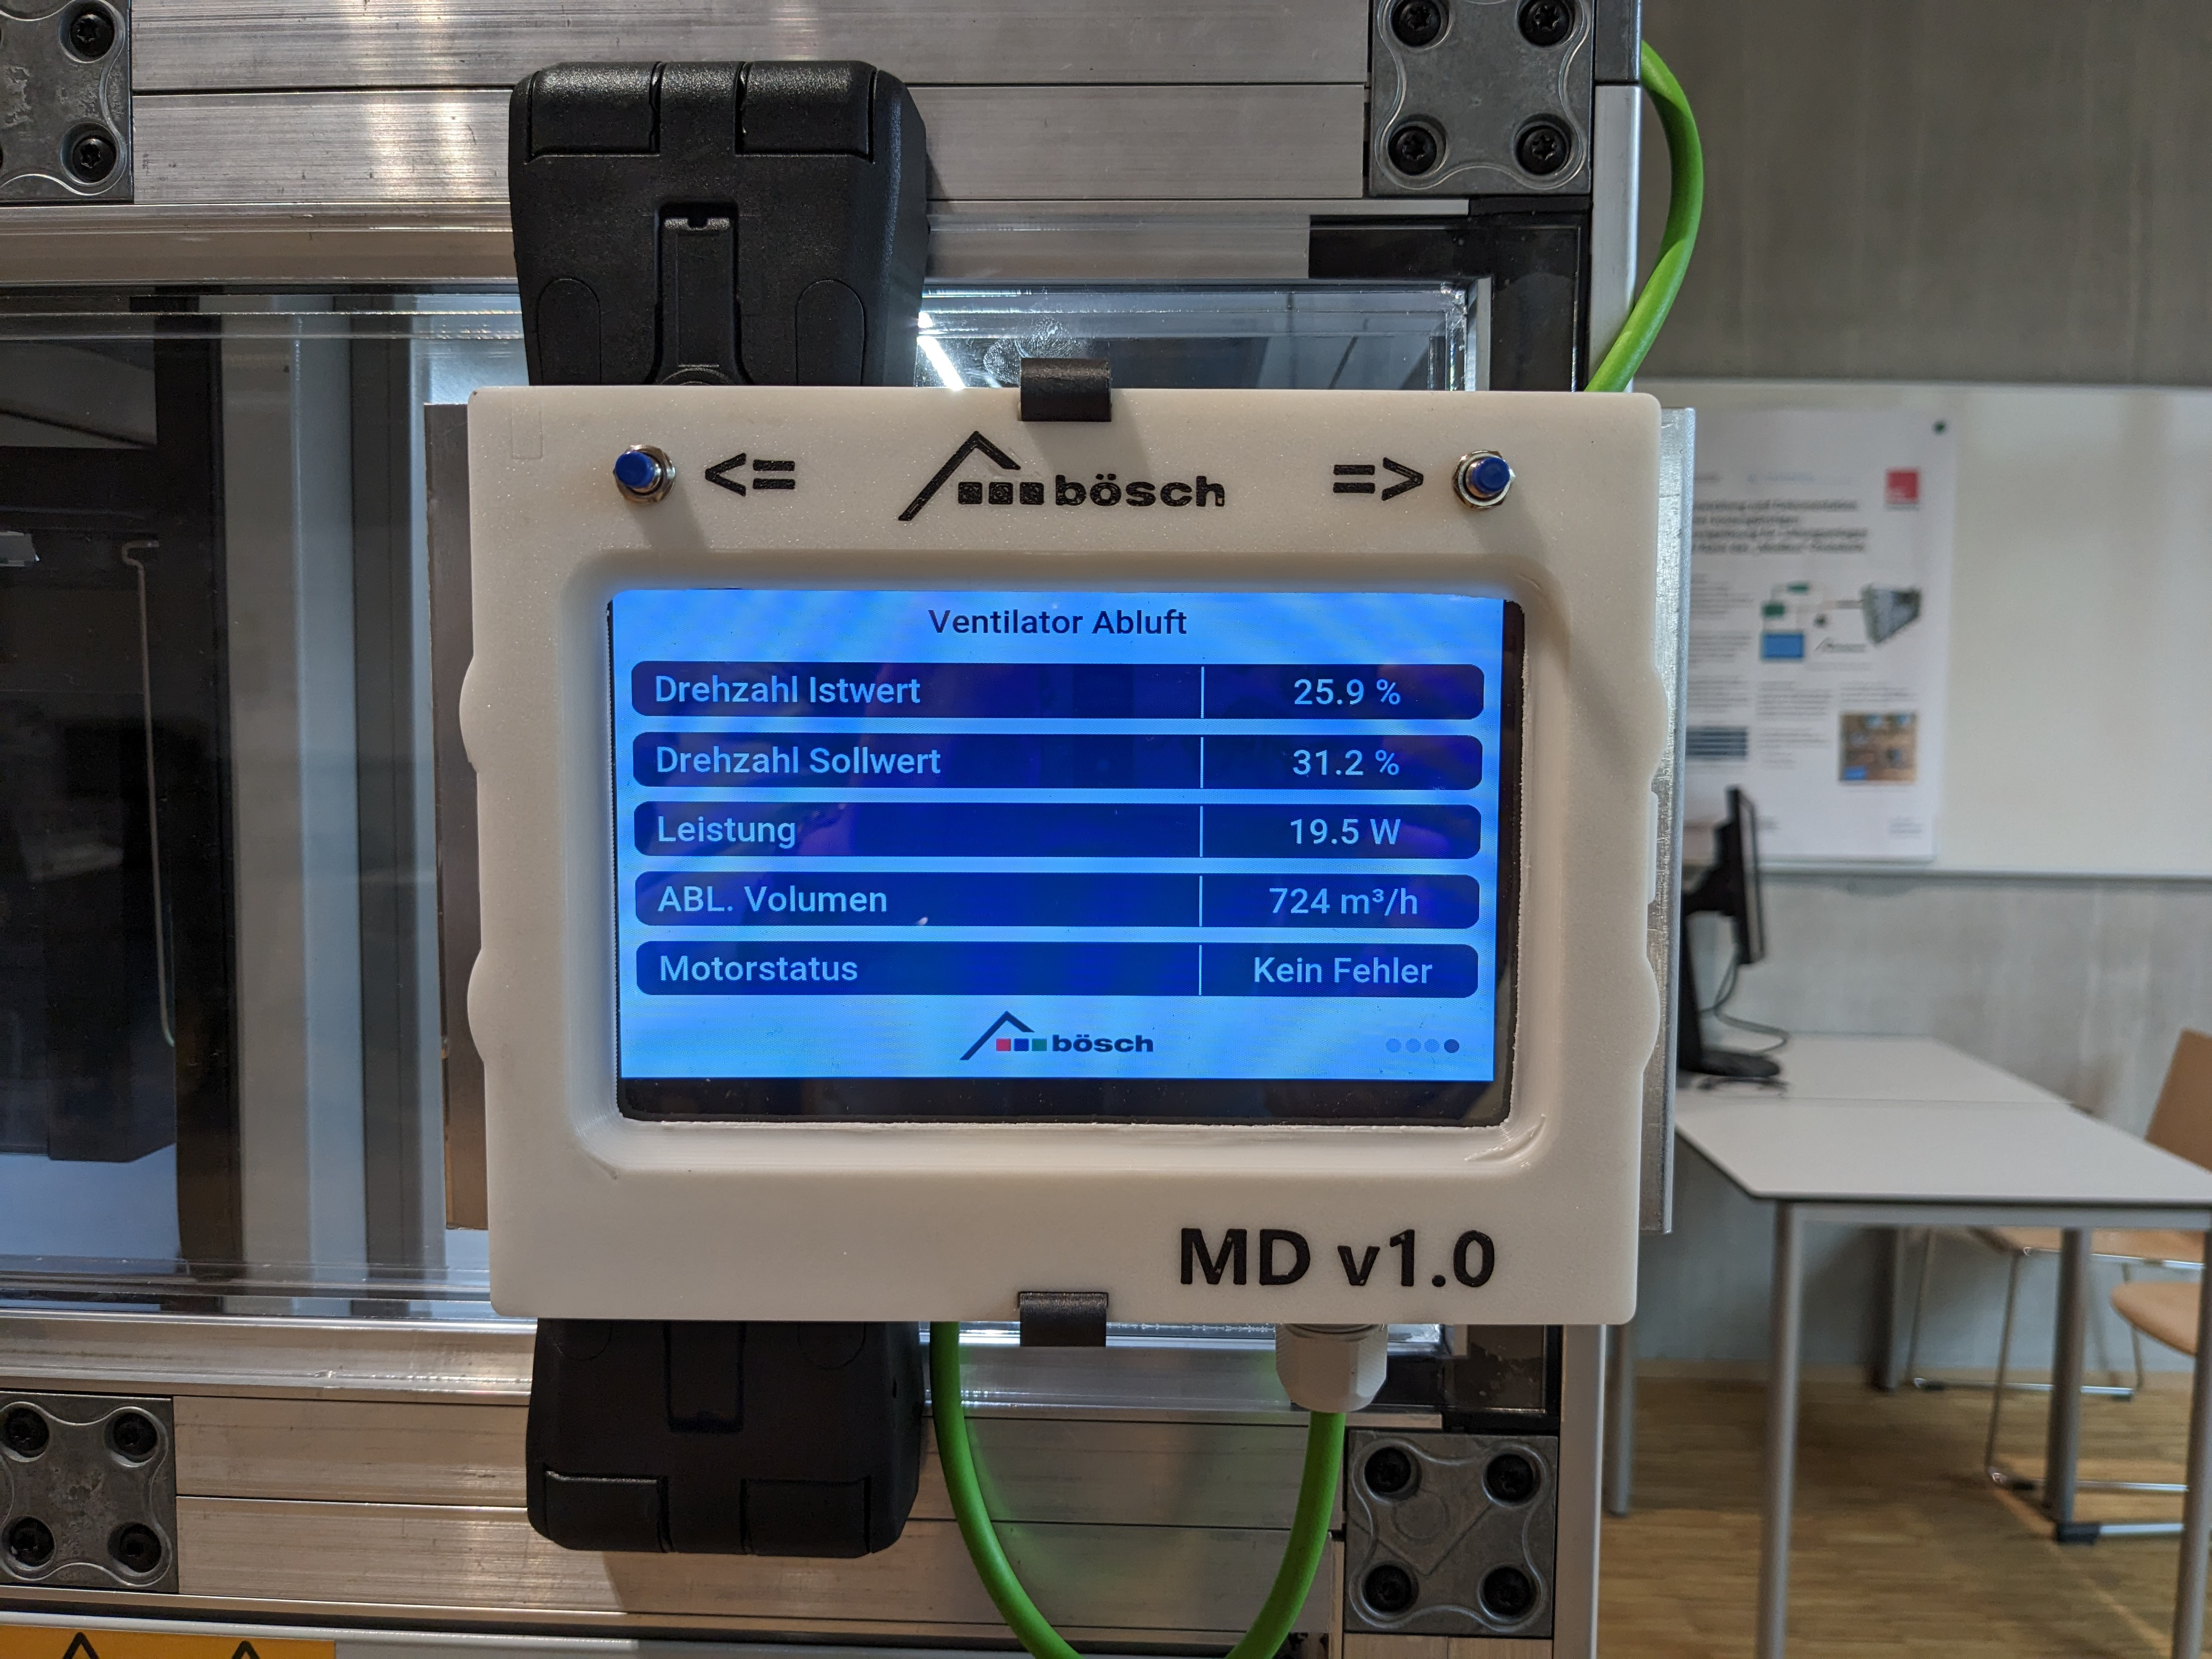
\includegraphics[width=0.7\linewidth]{Bilder/tdot_anzeige}
	\caption{\ac{rltanzeige} \gls{tdot} / Messe \ac{rltanlage}} 
	\label{fig:tdot_anzeige}
\end{figure}

In Abb.~\ref{fig:tdot_anzeige} sieht man die \ac{rltanzeige} konfiguriert für die \gls{tdot} \ac{rltanlage}. Auf der aktuell dargestellten Seite, sieht man den Status des \gls{abluft} Ventilator. Dabei werden die berechnete Ist Drehzahl angezeigt. Dazu der ausgegebene Drehzahl Sollwert und den aktuellen verbrauch an Leistung. An der 2. untersten Position befindet sich der Wert für die aktuell vom \gls{abluft} Ventilator geförderte Luftmenge. Auf der untersten Position wird der Motorstatus angezeigt, welcher keinen Fehler aufweist. Die \ac{rltanzeige} lässt sich mithilfe der gekennzeichneten Buttons weiter schalten um auf die anderen Ausgabeparameter zu kommen. Angeschlossen wird die \ac{rltanzeige} in diesem Fall mit dem grünen Modbuskabel. Sie wird direkt auf der Systemsteuerung der \ac{rltanlage} angeschlossen (fungiert als Erweiterung des internen Modbus Kabelbaum).

